\documentclass[russian,utf8,emptystyle,12pt]{eskdtext}
\usepackage[utf8]{inputenc}
\usepackage[T1,T2A]{fontenc}
\usepackage[russian]{babel}
\usepackage{wrapfig}
\usepackage{mathtext}
\usepackage{amsmath}
\usepackage{hyperref}
\usepackage{tabularx}
\usepackage{array} 

\setlength{\extrarowheight}{2pt}
\graphicspath{{img/}}

\title{Синтез регуляторов с помощью генетических алгоритмов}
\author{Кононенко~С.~А.}

\ESKDdepartment{Санкт-Петербургский Государственный Научно Исследовательский Университет Информационных Технологий Механики и Оптики}

\ESKDtitleDesignedBy{Автор}{Кононенко~С.~А.}
\ESKDtitleDesignedBy{Научный руководитель}{Бойков~В.~И.}
\ESKDtitleDesignedBy{Заведующий кафедрой}{Бобцов~А.~А.}

\begin{document}

    \maketitle
    
    \tableofcontents
    
    \section*{Введение}
    \addcontentsline{toc}{section}{Введение}	
    
		При разработке современных систем управления возникает проблема отсутствия явного аналитического решения поставленной задачи. Так при синтезе регулятора, обычно, к качеству системы устанавливают болшшое число противоречивых требований. Например, к времени переходного процесса, перерегулированию, допустимой ошибке, максимальному уровню сигнала, ограничению допустимых значений коэффициентов передачи, интервалу съема информации и так далее. Такие задачи могут быть решены методом поиска оптимального значения, в часности генетическим алгоритмом (ГА).
		
		В данной работе представленна разработка программного обеспечения (ПО) для синтеза пропорционального регулятора с использованием ГА поиска, а также определены основные свойства и параметры алгоритма.
		
		
	   
    \section{Формулировка проблемы}
    
        Рассмотрим объект управления, который описывается системой дифференциальных уравнений первого порядка в форме Коши~\cite{bib:miroshnik}.
        
        \begin{equation}
            \begin{cases}
                \dot x(t) = A x(t) + B u(t) \\
                     y(t) = C x(t) \\
            \end{cases}
            \label{eq:state-space}
        \end{equation}
        
	    \begin{ESKDexplanation}
	        \item[где ] $u$ - вектор (набор) входных переменных
	                    (воздействий);        
	        \item $y$ - вектор выходных переменных (управляемых величин);
	        \item $x$ - вектор переменных состояния (фазовых координат системы);
	        \item $A$ - матрица коэффициентов системы, характеризующая её
	                    внутренние свойства;
	        \item $B$ - матрица входных коэффициентов (матрица управления);
	        \item $C$ - матрица выходных коэффициентов.
        \end{ESKDexplanation}
        
        Пропорциональный регулятор формирует управление
        
        \begin{equation}
            u(t) = K x(t).
            \label{eq:control}
        \end{equation}
        
        Управление пропорционально измеряемым составляющим вектора состояния $x(t)$. Задача синтеза пропорционального регулятора является поиск коэффициентов закона управления $K$, при котором система будет удовлетворять заданным техническим требованиям.
        
        Будем синтезировать регулятор, исходя из следующих требований:
        
        \begin{enumerate}
        	\item Время переходного процесса $t_s$ --- должно быть минимально;
        	\item Задана величина допустимой ошибки системы, по одной из компонент вектора состояния (выходной величине)
        	
		        \begin{equation}
		            e < e_{max},
		            \label{eq:max-e}              
		        \end{equation}
		            
        	\item Заданы ограничения на области допустимых значений коэффициентов передачи регулятора
        	
		        \begin{equation}
		            K < K_{imax}, 
		            \label{eq:max-k}              
		        \end{equation}
		        
        \end{enumerate}
        
        Необходимо разработать процедуру поиска решения поставленной задачи с использованием ГА.
        
        
    
	\section{Программное обеспечение синтеза регулятора}	
	
	    Основным в задаче реализации генетического алгоритма является реализация целевой функции. Для данной задачи была разработано специальное ПО для моделирования динамических систем на основе GNU Scientific Library \cite{bib:air-fish, bib:gsl}. 
	    
	    Языком разработки ПО был выбран язык C. Так как язык С не является объектно ориентированным языком, классы и наследование симулировано с помощью структур и функций обработки каждой структуры. ПО состоит из двух частей: библиотека инструментов для моделирования динамики системы и библиотека компонентов алгоритма поиска.
	    
        \begin{figure}
            \centering
            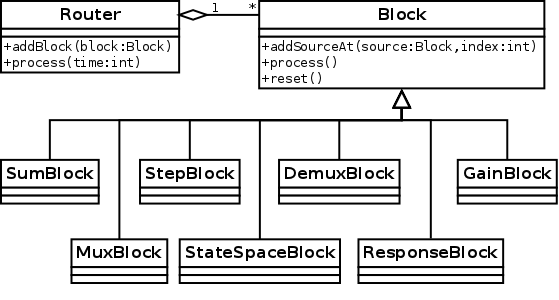
\includegraphics[scale=0.5]{simulating-classes.png}
            \caption{Диаграмма классов системы моделирования.}
            \label{fig:simulating-classes}
        \end{figure}	 
	    
	    Инструменты моделирования позволяют вычислить переходную характеристику системы с конкретным регулятором и проанализировать ее показатели качества. Основными сущностями билиотеки моделирования представлены на рисунке \ref{fig:simulating-classes}, ими являются "роутер" и "блок".
	    
	    Роутер представляет собой сущность, которая управляет временем моделирования и, в зависимости от топологии блоков, приемопередачей сигналов каждого блока.
	    
	    Блоки в свою очередь огранизуют топологию передачи сигнала. Конкретный блоки по разному реализуют обработку сигнала и имеет свои собственные параметры входов и выхода. Каждый блок в зависимоти от конкретной реализации обрабатывает входной и генерирует выходной сигнал. Если одна из функций блока не реализована, то он является либо только источником, либо только приемником (стоком) сигнала. Для успешного моделирования системы, должен существовать хотябы один блок-приемник.
        
        \begin{figure}[h!]
            \centering
            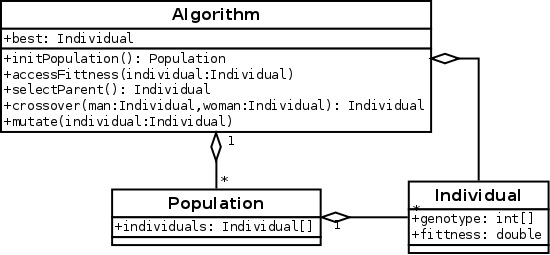
\includegraphics[scale=0.48]{ga-classes.png}
            \caption{Диаграмма классов генетического алгоритма.}
            \label{fig:ga-classes}
        \end{figure}
        
	    Компоненты генетического алгоритма поиска позволяют осуществить поиск оптимального решения комбинируя элементы случайного и градиентного поиска~\cite{bib:metaheuristics}. 
                        	    
        \begin{figure}[h!]
            \centering
            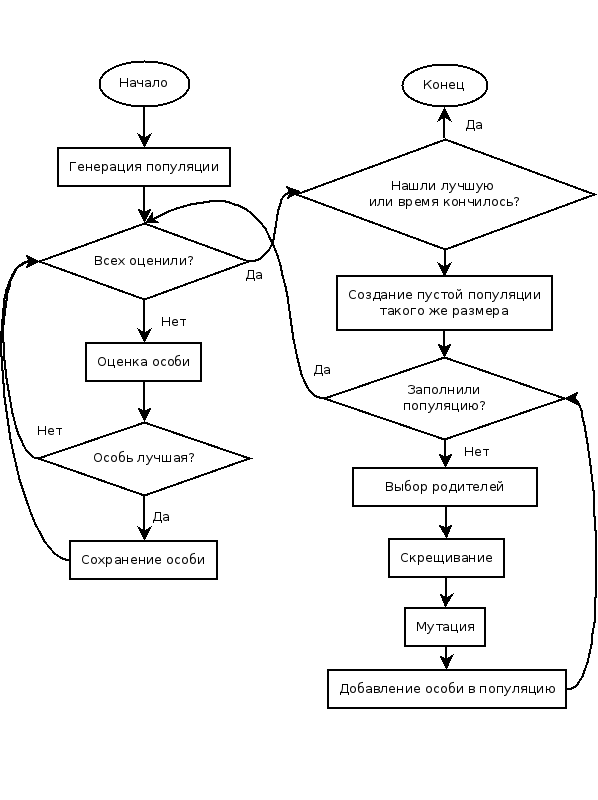
\includegraphics[scale=0.6]{ga.png}
            \caption{Генетический алгоритм.}
            \label{fig:ga}
        \end{figure}	
		
	    Основные сущности ГА представлены на рисунке~\ref{fig:ga-classes}. Поиск реализуется с помощью трёх сущностей: алгоритм, популяция и особь. Популяция предствляет собой множество особей, каждая из которых содержит генотип --- кандидат на решение задачи поиска. Алгоритм --- содержит собственно логику поиска оптимального решений, логика поиска  представлена на рисунке~\ref{fig:ga} и содержит в себе следующие основные действия~\cite{bib:metaheuristics}:
                	    
        \begin{enumerate}
            \item Генерация исходной популяции;
            \item Оценка особи;
            \item Выбор родителя;
            \item Скрещивание;          
            \item Мутация.         
        \end{enumerate}
                
    	Для конкретной задачи генерация исходной популяции представляет собой выбор N-ного числа случайных векторов из области 
    	
        \begin{equation}
           K_o = [-K_{imax}, K_{imax}], 
           \label{eq:search-area}       
        \end{equation} 
        
        что соответствует условию~\ref{eq:max-k}.
	    
	    \begin{figure}[h!]
	        \centering
	        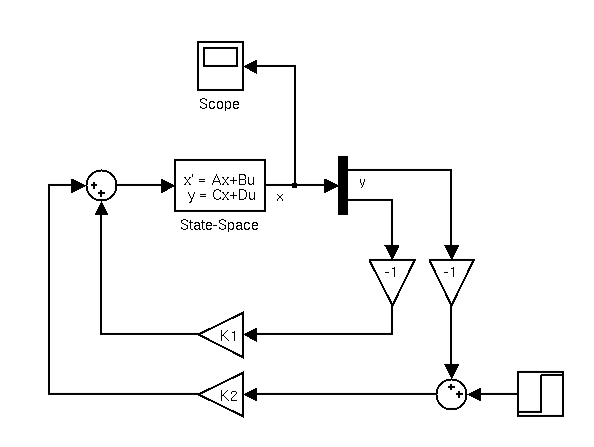
\includegraphics[scale=0.5]{simulation.png}
	        \caption{Схема моделирования системы.}
	        \label{fig:simulation}
	    \end{figure}
            	
    	Для оценки особи производится моделирование системы представленной на рисунке \ref{fig:simulation}, на которой блоки усиления К1 и К2 соотвествуют составляющим вектора $K$. После моделирования с помощью блока анализа переходной функции определяется время стабилизации. Границы сигнала для времени стабилизации соответствуют условию максимальной ошибки \ref{eq:max-e}.
                    
        Полученное время переходного процесса используется для определения приспособленности особи по формуле:
                    
        \begin{equation}
           F = (\frac{1}{t_s} + c)^2,     
           \label{eg:fittness}   
        \end{equation} 
        
 	    \begin{ESKDexplanation}
            \item[где ] $c$ - константа, устанавливающая минимальную приспособленность особи.    
        \end{ESKDexplanation}
            
    	Выбор родителя в генетическим алгоритме должен решать две основные задачи: cохранение лучших особей и избежание вырождения. Для решения обеих задач используется следующий алгоритм. Каждой особи  на числовой оси ставиться в соответствие отрезок, размер которого пропорционален оценки особи. Затем случайным образом выбирается число на этой числовой оси. Особь которой соответствует выбранный отрезок выбирается для скрещивания.
            
		Для скрещивания, в связи с малыми размерами генотипа, был выбран пособ случайной перестановки составляющих родительских векторов.
            
		Мутация выражается фомулой:
                        
        \begin{equation}
           K_{im} = K_i * (1 + m * R), 
           \label{eg:mutation}   
        \end{equation}    
                     
 	    \begin{ESKDexplanation}
            \item[где ] $K_{im}$ --- новое значение составляющей вектора,
            \item       $K_i$ --- старое значение составляющей вектора,
            \item       $R$ --- равномерно распределённая в интервале $[-1, 1]$ случайная величина,
            \item       $m$ --- коэффициент мутации,     
        \end{ESKDexplanation}
                    
        при условии что новые значения удовлетворяет условию \ref{eq:max-k}.
	    
	    
	\section{Проверка работоспособности программного обеспечения}    
	    
	    Работоспособность разработанного ПО была проверена на задаче синтеза пропорционального регулятора для объекта управления второго порядка. В результате синтеза необходимо найти значения коэффициентов закона управления~\ref{eq:control} $K = [ K_1, K_2 ]$, соответсвующие условиям \ref{eq:max-k} и \ref{eq:max-e}:
	    
    	\begin{eqnarray}
    		\left| K_1 \right| < 100 \label{eq:max-k1} \\
    		\left| K_2 \right| < 100 \label{eq:max-k2} \\
    		e < 1\%
    	\end{eqnarray}
    	
		В ходе проведения машинных экспериментов было отмечено следующее.
		
      	Время расчета влияет на оценку приспособленности особи в популяции. Уменьшение этого времени ведет к увеличению локальности поиска так как особи с большим временем переходного процесса окажутся оценены так же, как и особи с неустойчивым характером поведения. Время расчета переходного процесса варьировалось от 10 до 30 с.
                  
      	Шаг моделирования очевидным образом влияет на точность оценки, поэтому принципиально не влияет на оптимальное решение. В данной работе шаг составил 0.05 с.
                                   
      	Важным параметром алгоритма является число особей в популяции. Основная задача этого параметра -- выявить в первой популяции особей с оценкой выше минимальной. При выполнении данного условия, градиентная составляющая поиска получит возможность направленного движения. Для поиска решений в обсласти заданной ограничениями \ref{eq:max-k1} и \ref{eq:max-k2} достаточное число особей равное 100.
                 
      	Минимальная приспособленность особи параметр влияет на возможность особи участвовать в скрещивании. При существенном увеличении данного параметра, поиск смещается в сторону случайного поиска, что увеличивает время поиска решения. В данной работе $c = 0.001$.

      	Коэффициент мутации является основным параметром градиентной составляющей поиска. Диапаон возможной мутации влияет на плавность схождения к результату. В данной работе $m = 0.05$.
                  
      	Время поиска является основным ограничивающим фактором цикла поиска решений. Поэтому для различных типов сходимости к результату выбирается подходящее время. В проведенных экспериметах время варьировалось от 1 до 3 минут. За это время проводилос от 5 до 10 генераций новых популяций. В зависимости от них меняется скорость поиска и качество найденного решения. 
      
      	На рисунках \ref{fig:result-1}, \ref{fig:result-2} и \ref{fig:result-3} ипоказаны типовые переходные характеристики синтезируемых регуляторов для трех объектов с различной динамикой.
      
	  	\begin{eqnarray}
			A_1 =& \left| \begin{array}{cc} -0.45 & 1 \\ -0.05 & 0 \end{array} \right|,
		    &B_1 = \left| \begin{array}{c} 0 \\ 0.1 \end{array} \right|. 
		    \label{eq:system-1} \\   
			A_2 =& \left| \begin{array}{cc} 1 & 5 \\ 2 & 1 \end{array} \right|,
		    &B_2 = \left| \begin{array}{c} 0 \\ 1 \end{array} \right|. 
		    \label{eq:system-2} \\   
			A_3 =& \left| \begin{array}{cc} 0 & 1 \\ -15 & -5 \end{array} \right|,
		    &B_3 = \left| \begin{array}{c} 0 \\ 1 \end{array} \right|. 
		    \label{eq:system-3}  
		\end{eqnarray}

		\begin{figure}[h]
		    \centering
		    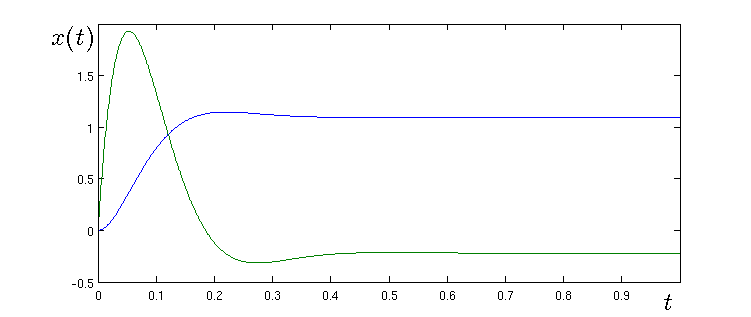
\includegraphics[scale=0.65]{result_1.png}
		    \caption{Моделирование системы \ref{eq:system-1} с регулятором.}
		    \label{fig:result-1}
		\end{figure}
		    
		\begin{figure}[h]
		    \centering
		    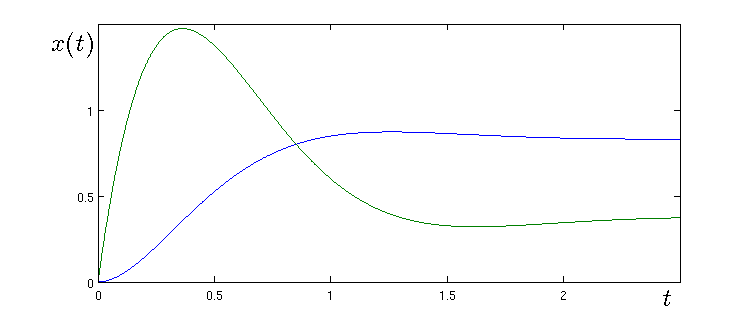
\includegraphics[scale=0.65]{result_2.png}
		    \caption{Моделирование системы \ref{eq:system-2} с регулятором.}
		    \label{fig:result-2}
		\end{figure}
		    
		\begin{figure}[h]
		    \centering
		    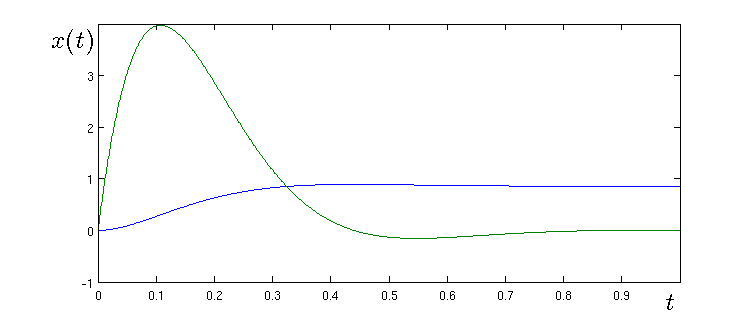
\includegraphics[scale=0.65]{result_3.png}
		    \caption{Моделирование системы \ref{eq:system-3} с регулятором.}
		    \label{fig:result-3}
		\end{figure}
        
    	При различии времени переходного процесса на порядок время поиска оптимального решения остается примерно одинаковым.
        


	\section*{Заключение}
  	\addcontentsline{toc}{section}{Выводы}	
    
    	Разработанное программное обеспечение позволяет производить синтез регуляторов на базе генетических алгоритмов. Алгоритм сходится при условиии наличия оптимального решения. Конечное время сходимости обеспечивает наличие в первой популяции особи с оценкой выше минимальной.
    
    	Полученный результат свидетельствует о возможности дальнейшего развития и применения генетических алгоритмов в задачах управления.
    


	\bibliography{index}{}
	\bibliographystyle{plain}
  
\end{document}
